%
% File naacl2019.tex
%
%% Based on the style files for ACL 2018 and NAACL 2018, which were
%% Based on the style files for ACL-2015, with some improvements
%%  taken from the NAACL-2016 style
%% Based on the style files for ACL-2014, which were, in turn,
%% based on ACL-2013, ACL-2012, ACL-2011, ACL-2010, ACL-IJCNLP-2009,
%% EACL-2009, IJCNLP-2008...
%% Based on the style files for EACL 2006 by 
%%e.agirre@ehu.es or Sergi.Balari@uab.es
%% and that of ACL 08 by Joakim Nivre and Noah Smith

\documentclass[11pt,a4paper]{article}
\usepackage[hyperref]{naaclhlt2019}
\usepackage{times}
\usepackage{latexsym}

\usepackage{tabularx}
\usepackage{amssymb}
\usepackage{amsmath}
\usepackage{latexsym}
\usepackage{enumitem}
\usepackage{booktabs}
\usepackage{url}
\usepackage{color} 
\usepackage{verbatim}
\usepackage{calc}
\usepackage{arydshln}
\setlength\dashlinedash{0.7pt}
\setlength\dashlinegap{1.pt}
\setlength\arrayrulewidth{0.3pt}
\usepackage{mathtools}
\usepackage[draft]{todonotes}
\newcommand{\raq}[1]{\textcolor{blue}{R: #1}}
\newcommand{\marco}[1]{\textcolor{red}{M: #1}}
\newcommand{\gbt}[1]{\textcolor{green}{G: #1}}
\newcommand{\redd}{Reddit$_{13}$}
\usepackage{soul}



%\aclfinalcopy % Uncomment this line for the final submission
%\def\aclpaperid{***} %  Enter the acl Paper ID here

%\setlength\titlebox{5cm}
% You can expand the titlebox if you need extra space
% to show all the authors. Please do not make the titlebox
% smaller than 5cm (the original size); we will check this
% in the camera-ready version and ask you to change it back.

\newcommand\BibTeX{B{\sc ib}\TeX}

\title{Short-term meaning shift: an exploratory distributional analysis\\
\vspace*{0.5cm}
Supplementary Material}

\author{First Author \\
  Affiliation / Address line 1 \\
  Affiliation / Address line 2 \\
  Affiliation / Address line 3 \\
  {\tt email@domain} \\\And
  Second Author \\
  Affiliation / Address line 1 \\
  Affiliation / Address line 2 \\
  Affiliation / Address line 3 \\
  {\tt email@domain} \\}

\date{}

\begin{document}
\maketitle
%============================

%% first page
%
%\begin{minipage}{15cm}
%Included in this file are the following supplementary materials:
%\begin{itemize}
%\item Pages 2: details of the survey.
%\item Pages 3--5: the survey instructions provided to the redditors.
%\item Page 6: the scatterplot representing the correlation between contextual variability and semantic shift.
%
%\end{itemize}
%
%\end{minipage}
%
%\pagebreak
%\clearpage

%============================

% first page

\section{Further details on Data and Model}
We downloaded Reddit data using the Python package Praw: \url{https://pypi.python.org/pypi/praw/}.

The model was implemented using the Python package Gensim: \url{https://pypi.python.org/pypi/gensim/}.

\section{Further details on Evaluation Dataset}

For our experiment, we considered content words only, which we identified by using the external list of common words available at \url{https://www.wordfrequency.info/free.asp}.

As detailed in the main paper, 26 members of r/LiverpoolFC participated in the survey, and each word received on average 8.8 judgements. We computed inter-annotator agreement as Krippendorff's alpha, and obtained $\alpha$ = 0.58, a relatively low value but common in semantic tasks \cite{artstein2008inter}.

The survey included 3 main groups of words:  
(1) words with no frequency increase between $t_1$ and $t_2$; 
(2) words marked as semantic shift candidates by the authors; 
(3) words with a significant increase in frequency but not marked as meaning
shift candidates.
The analysis of the shift index based on redditors' annotation shows that words in group 1 have an average shift index of 0.07 ($\pm$ 0.12) - a result which validates our data selection method. For words belonging to group 2 the average shift index is 0.72 ($\pm$ 0.15), while for those in group 3 is 0.15 ($\pm$ 0.16).


%\pagebreak
\clearpage

%============================

% table for section 5.2
\begin{minipage}{15cm}

\textbf{Survey's Instructions}. Below the instructions provided to the participants in the survey.

\vspace*{0.5cm}

\paragraph{What is this about?}
Words can acquire new meanings in short periods of time. Think about the word `insane': until recently, it was only used in a negative way to say someone or something was mad. In the last couple of years, it has flipped its sense, and you can find it in sentences like: `Salah scored an insane goal', meaning that the goal was amazing.
Changes of meaning like this are very frequent, especially in the slang language used in online communities. The goal of this survey is to identify words that have recently changed their meaning in the r/LiverpoolFC subreddit.
\\
\paragraph{What is this about?}
You will be presented with a set of target words. For each word, you will be shown a few posts from r/LiverpoolFC where the word is used. Some of the posts date back to 2011-2013, while the others have been written in 2017.
We ask you to indicate whether the meaning of the word (the way the word is used) has changed between 2011-2013 and 2017. There are no right or wrong answers: we are interested in your opinion given you personal experience as a member of the subreddit and your observation of the sample posts. Please make a choice, even if it is difficult or unclear. If you have comments about a word, feel free to include them in the comment box. In the next page you will see some examples, coming from other communities of football fans, so you can practice, and then the actual survey will start. You can exit the survey at any moment pressing the `finish' bottom. 

\vspace*{0.5cm}

\textbf{Example 1}

\vspace*{0.5cm}

Target word: \textbf{CAN}

\vspace*{0.25cm}
2011-2013
\begin{itemize}
\item We begin by drinking a warm \textbf{can} of Diet Coke
\item What? Opened the \textbf{can} and poured it out
\item Not even an empty beer \textbf{can}
\end{itemize}

\vspace*{0.25cm}

2017
\begin{itemize}
\item In today's match we are wearing the \textbf{can}
\item The apple pie, whipped cream, followed by downing a \textbf{can} of beer
\item Hapoel-Inter 3-2: players suck when playing with that \textbf{can} kit...
\end{itemize}

\vspace*{0.25cm}

\textbf{[X}] \textbf{change}: there is at least one post in 2017 where the meaning of the word is novel and different from 2011-2013

[  ] \textbf{no change}: the meaning is the same in 2011-2013 and 2017

\vspace*{0.25cm}

In the example above, it makes sense to select change because in 2011-2013 the target word `can' is always used with its standard meaning, while in posts 1 and 3 of  2017 it is used to talk about the third kit of the Team, whose colors recalled those of a Sprite can. Due to this similarity, the fans started to call that kit just the `can'. 
Note: it's enough for one or two of the examples from 2017 to show a novel meaning for you to choose the change option.

\end{minipage}

\pagebreak

\clearpage

%============================

\begin{minipage}{15cm}

\textbf{Example 2}

\vspace*{0.5cm}

Target word: \textbf{TRANSFER}

\vspace*{0.25cm}
2011-2013
\begin{itemize}
\item One thing Jose will improve for sure is \textbf{transfer} policy
\item United believe they will be able to negotiate \textbf{transfer} fees down
\end{itemize}

\vspace*{0.25cm}

2017
\begin{itemize}
\item Yeah we've nailed last \textbf{transfer} window
\item they're both strikers arriving on a free \textbf{transfer} who are at the end of their careers
\end{itemize}

\vspace*{0.25cm}

[  ] \textbf{change}: there is at least one post in 2017 where the meaning of the word is novel and different from 2011-2013

\textbf{[X}]  \textbf{no change}: the meaning is the same in 2011-2013 and 2017

\vspace*{0.25cm}

In this case, no change would be the appropriate answer. The meaning of the word "transfer" (move to another team) seems approximately the same in 2011-13 and 2017.

\vspace*{1.5cm}

\textbf{Example 3}

\vspace*{0.5cm}

Target word: \textbf{KID}

\vspace*{0.25cm}
2011-2013
\begin{itemize}
\item Come on bro, I am a real fan, since I was a \textbf{kid}
\item He's only 19 wow, people are worried about him not getting play time but this \textbf{kid} is still so young, his chance will come
\end{itemize}

\vspace*{0.25cm}

2017
\begin{itemize}
\item I was there! The \textbf{kid} scored first if not mistaken
\item should have been 1-3, the \textbf{kid} missed an easy chance
\end{itemize}

\vspace*{0.25cm}

\textbf{[X}]  \textbf{change}: there is at least one post in 2017 where the meaning of the word is novel and different from 2011-2013

[  ] \textbf{no change}: the meaning is the same in 2011-2013 and 2017

\vspace*{0.25cm}

In this case, the target word shows a change. In 2011-2013, `kid' is used with its standard meaning (child or youngster). However, in the posts from 2017 the word has become similar to a nickname: `kid' is the word fans in this group used to call a specific player.
\end{minipage}

\pagebreak

\clearpage

%============================

\begin{minipage}{15cm}

\textbf{Example 4}

\vspace*{0.5cm}

Target word: \textbf{BEER}

\vspace*{0.25cm}
2011-2013
\begin{itemize}
\item I was watching the game accompanied only with a bottle of \textbf{beer} and I fell asleep
\item Have a great day and fingers crossed we'll smash these off, have a \textbf{beer} for me!
\end{itemize}

\vspace*{0.25cm}

2017
\begin{itemize}
\item \textbf{Beer} and Sheva: what a wonderful night for Milan fans!
\item Inter had three \textbf{Beer} and get drunk in Europa League
\item And for Inter: \textbf{BEER BEER BEER}!!
\end{itemize}

\vspace*{0.25cm}

\textbf{[X}]  \textbf{change}: there is at least one post in 2017 where the meaning of the word is novel and different from 2011-2013

[  ] \textbf{no change}: the meaning is the same in 2011-2013 and 2017

\vspace*{0.25cm}

Another change example. In the posts from 2011-2013, `beer' is used with its standard meaning (to refer to the drink). But this is not so in the posts from 2017: when InterFC unpredictably lost the Europa League game to Hapoel Be'er Sheva fans of the other Italian teams transformed `Be'er' into `beer' and made a lot of jokes with this word, which was suddenly transformed into a \textit{meme}.
\vspace*{1.5cm}

\textbf{Example 5}

\vspace*{0.5cm}

Target word: \textbf{BOX}

\vspace*{0.25cm}
2011-2013
\begin{itemize}
\item We can deal with any cross they put into the \textbf{box}
\item just don't let them play passes in and around the \textbf{box}
\end{itemize}

\vspace*{0.25cm}

2017
\begin{itemize}
\item Good player, he’s a true \textbf{box} to \textbf{box}
\item Pretty realistic and outside-the-\textbf{box} thinking on my part
\end{itemize}

\vspace*{0.25cm}

[  ]\textbf{change}: there is at least one post in 2017 where the meaning of the word is novel and different from 2011-2013

\textbf{[X}] \textbf{no change}: the meaning is the same in 2011-2013 and 2017

\vspace*{0.25cm}

In this case, no change would be appropriate. In the posts from 2011-13 and in post 1 from 2017, `box' is used to indicate the penalty area. Therefore, its meaning has not changed. Note: In post number 2 from 2017, `box' is used as part of a common English expression. This use is not novel and hence does not indicate a change
\end{minipage}

\pagebreak

\clearpage

%============================

%\begin{minipage}{15cm}
%
%\textcolor{red}{REMOVE THIS IF YOU LEAVE IT IN THE MAIN PAPER}
%
%%\begin{figure}%[t]\centering
%%\includegraphics[width=\columnwidth]{graph_and_csv/plots/shift-cosine-correlation-plot.png}
%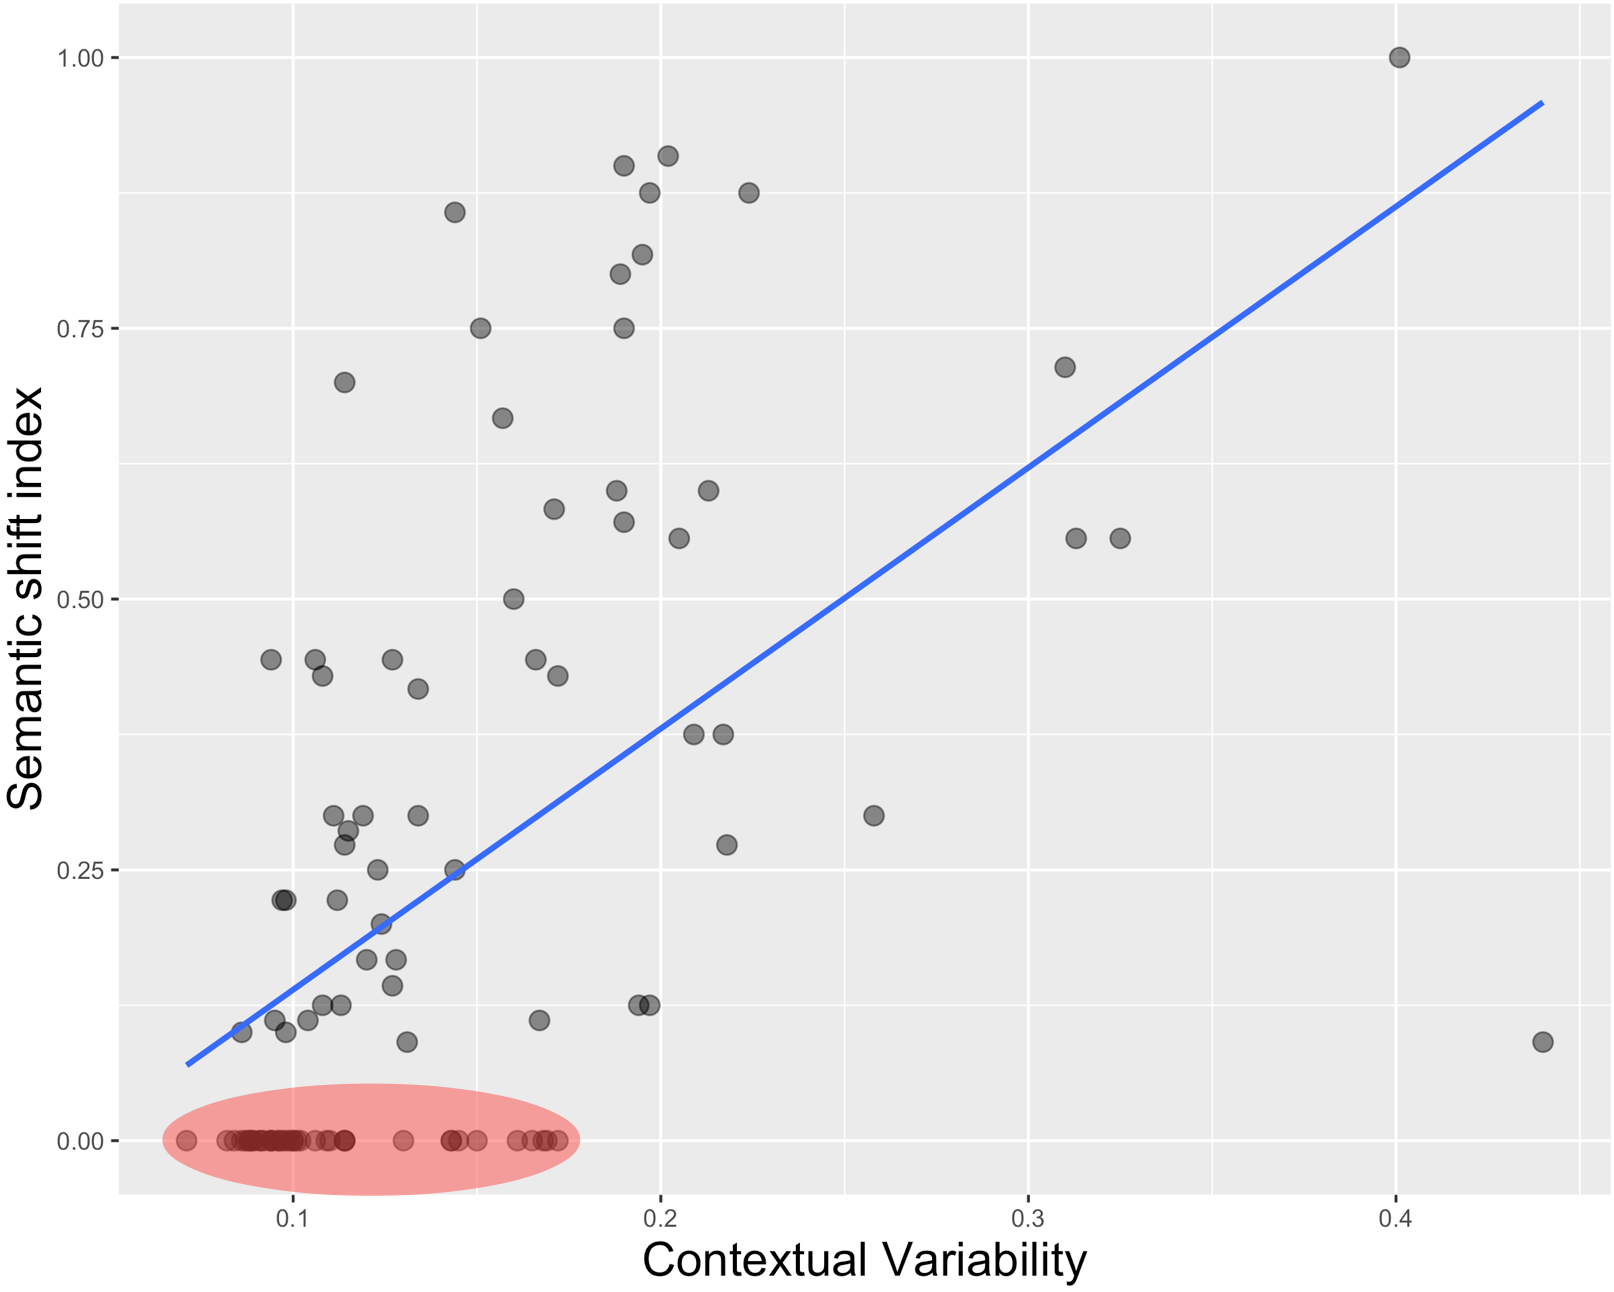
\includegraphics[width=\columnwidth]{images/contextual_variability_shift_index_annotated.png}
%
%\vspace*{0.25cm}
%
%Semantic shift index vs.~context variability for all words in the evaluation dataset (Pearson's $r$ = 0.55, $p< 0.001$). Red ellipses indicates the referential cases which are incorrectly assigned high cosine distance values (false positives in the paper).
%%\label{fig:shift-variability}}
%%\end{figure}
%
%
%\end{minipage}
%
%\pagebreak
%
%\clearpage

\bibliography{naaclhlt2019}
\bibliographystyle{acl_natbib}

%============================
%============================
%============================
\end{document}

%%% Local Variables:
%%% mode: latex
%%% TeX-master: t
%%% End:

